\documentclass[supercite]{Experimental_Report}

\title{并行编程与设计实验报告}
\school{计算机科学与技术学院}
\author{Sukuna}
\classnum{计算机校交1902班}
\stunum{U2019114514}
\instructor{金海} % 李平、孙伟平、范晔斌、陈加忠
\usepackage{zhnumber} % change section number to chinese
\renewcommand\thesection{\zhnum{section}}
\renewcommand \thesubsection {\arabic{subsection}}
\usepackage{tikz}
\usetikzlibrary{mindmap,trees}
\usepackage{algorithm, multirow}
\usepackage{algpseudocode}
\usepackage{amsmath}
\usepackage{amsthm}
\usepackage{framed}
\usepackage{mathtools}
\usepackage{subcaption}
\usepackage{amsmath, amssymb, amsfonts}
\usepackage{tabu}
\usepackage{xltxtra} %提供了针对XeTeX的改进并且加入了XeTeX的LOGO, 自动调用xunicode宏包(提供Unicode字符宏)
\usepackage{bm}
\usepackage{longtable}
\usepackage{tikz}
\usepackage{tikzscale}
\usepackage{pgfplots}
%\usepackage{enumerate}
\usepackage{graphicx}
\pgfplotsset{compat=1.16}

\newcommand{\cfig}[3]{
  \begin{figure}[htb]
    \centering
    \includegraphics[width=#2\textwidth]{images/#1.tikz}
    \caption{#3}
    \label{fig:#1}
  \end{figure}
}

\newcommand{\sfig}[3]{
  \begin{subfigure}[b]{#2\textwidth}
    \includegraphics[width=\textwidth]{images/#1.tikz}
    \caption{#3}
    \label{fig:#1}
  \end{subfigure}
}

\newcommand{\xfig}[3]{
  \begin{figure}[htb]
    \centering
    #3
    \caption{#2}
    \label{fig:#1}
  \end{figure}
}

\newcommand{\rfig}[1]{\autoref{fig:#1}}
\newcommand{\ralg}[1]{\autoref{alg:#1}}
\newcommand{\rthm}[1]{\autoref{thm:#1}}
\newcommand{\rlem}[1]{\autoref{lem:#1}}
\newcommand{\reqn}[1]{\autoref{eqn:#1}}
\newcommand{\rtbl}[1]{\autoref{tbl:#1}}

\algnewcommand\Null{\textsc{null }}
\algnewcommand\algorithmicinput{\textbf{Input:}}
\algnewcommand\Input{\item[\algorithmicinput]}
\algnewcommand\algorithmicoutput{\textbf{Output:}}
\algnewcommand\Output{\item[\algorithmicoutput]}
\algnewcommand\algorithmicbreak{\textbf{break}}
\algnewcommand\Break{\algorithmicbreak}
\algnewcommand\algorithmiccontinue{\textbf{continue}}
\algnewcommand\Continue{\algorithmiccontinue}
\algnewcommand{\LeftCom}[1]{\State $\triangleright$ #1}


\newtheorem{thm}{定理}[section]
\newtheorem{lem}{引理}[section]
\renewcommand {\thefigure} {\arabic{figure}}
\colorlet{shadecolor}{black!15}

\theoremstyle{definition}
\newtheorem{alg}{算法}[section]
\def\thmautorefname~#1\null{定理~#1~\null}
\def\lemautorefname~#1\null{引理~#1~\null}
\def\algautorefname~#1\null{算法~#1~\null}
\usepackage{xcolor}
\usepackage{listings}
\usepackage[skins]{tcolorbox}
\tcbuselibrary{breakable}
\newtcolorbox{abox}[1][]{enhanced,
	fonttitle = \heiti \large \bfseries,% 标题字体设置
	colbacktitle =black,% 标题背景颜色
	coltitle=white,% 标题字体颜色
	% halign title=center,% 标题对齐方式
	attach boxed title to top left = {yshift = -5pt},
	%	将标题以box 形式放在文本框左上角,并向下移动5pt	
	%----------正文字体--------
	fontupper = \kaishu,%正文字体设置
	%colback = white,%正文背景颜色设置
	%---------边框设置---------
	arc = 4pt,%正文边框边角弧度
	%	boxed title style={arc=0pt},%标题框边角弧度
	colframe=black,%边框颜色设置
	toprule  = 1pt,%取消上边框
	rightrule = 1pt,%取消下边框
	%---------调整字体位置------
	top = 10pt,%增大正文文本与上边框距离
	%---------设置标题为默认参数,不影响其他参数的设置
	title=#1,
	breakable
}
\newcommand{\tabincell}[2]{\begin{tabular}{@{}#1@{}}#2\end{tabular}}  
\begin{document}

\maketitle
\clearpage

\pagenumbering{Roman}

\tableofcontents[level=2]
\clearpage

\pagenumbering{arabic}
\section{实验一}
\subsection{串行环境下的排序算法}
\subsubsection{实验目的与要求}

在串行环境下编写串行排序的C语言小程序,并按要求输出对应的排序结果。串行排序方法任选。

\subsubsection{算法描述}
在本实验中我使用的排序算法为快速排序,有关快速排序算法的描述见算法\ref{alg:F1}
\begin{algorithm}[htb]
\caption{快速排序}
\label{alg:F1}
\hspace*{0.02in} {\bf Input:}
数组的个数n以及n个数组元素\\
\hspace*{0.02in} {\bf Output:} 
升序排序之后的数组
\begin{algorithmic}[1] 
\State 首先设定一个分界值,通过该分界值将数组分成左右两部分
\State 将大于或等于分界值的数据集中到数组的右边,小于分界值的数据集中到数组的左边。此时,左边部分中各元素都小于分界值,而右边部分中各元素都大于或等于分界值
\State 左边和右边的数据可以独立进行排序。对于左侧的数据,又可以取一个分界值,将该部分数据分成左右两部分,右侧的数据也可以做类似的处理
\State 重复上述过程,直到排序完成
\end{algorithmic}
\end{algorithm}

\subsubsection{复杂度分析}
快速排序通过partition操作将长度将长度为n的数组分成3部分,假设左边有i个元素,右边有n-1-i个元素,中间的基准值为pivot。假设所有可能的输入等概率出现,那么所有的划分情况也会等概率出现,即i会以相等的概率取区间[0, n-1]中的每一个值,所以快速排序的平均时间复杂度为
$$ A[n] = \underbrace{n-1}_{cost \ of \ partition}+\underbrace{\sum_{i = 0}^{n-1}\frac{1}{n}[A(i) + A(n-1-i)]}_{cost \ of \ left \ and \ right \ parts},n \ge 2 $$

递归的初始情况:A[1]=A[0]=0,另外可以注意到左右两部分递归具有对称性,所以有
$$ \sum_{i=0}^{n-1}A(i)=\sum_{i=0}^{n-1}A(n-1-i)$$

于是上述公式可以简化成如下形式:
$$ A(n)=(n-1)+\frac{2}{n}\sum_{i=0}^{n}A(i) $$

于是到了熟悉的数列求通项公式环节,以下为数学推导,采用错位相减法
\begin{equation*}
    \begin{split}
    & nA(n)-(n-1)A(n-1)=n(n-1)+2\sum_{i=0}^{n-1}A(i)\\
    &\Longrightarrow nA(n)=(n+1)A(n-1)+2(n-1)\\
    &\Longrightarrow \frac{A(n)}{n+1}=\frac{A(n-1)}{n} + \frac{2(n-1)}{n(n+1)} 
    \end{split}
\end{equation*}

考虑初始情况B(1)=B(0)=0,接下来求解这个数列通项
\begin{equation*}
    \begin{split}
        & B(n)=B(n-1)+\frac{4}{n+1}-\frac{2}{n}\\
        & \Longrightarrow B(n)-\frac{2}{n+1}=B(n-1)-\frac{2}{n}+\frac{2}{n+1}
    \end{split}
\end{equation*}

令 $C(n) = B(n) - \frac{2}{n+1}$,于是有$C(n) = C(n-1)+\frac{2}{n+1}$,初始情况为$C(1)=-1,C(0)=-2$,所以$C(n) = \sum_{i=0}^{n}\frac{2}{i+1}=O(logn)$,所以$B(n)=O(logn)$,$A(n) = (n+1)B(n) = O(nlogn)$,从而我们得知了快速排序的时间复杂度为$O(nlogn)$

程序中仅开辟了一个一维数组对数据进行保存,易知快速排序程序的空间复杂度为$O(n)$。

\subsubsection{实验结果和分析}
输入数据:8 49 38 65 97 76 13 27 49

快速排序过程如下:

$\{\color[rgb]{1,0,0}{49}$
$,38,65,97,76,13,27,49\}$

第一次划分之后:

$\{27,38,13\},\color[rgb]{1,0,0}{49}$
$,\{76,97,65,49\}$

左部数据继续排序

$\{13\},$
$\color[rgb]{1,0,0}{27}$
$,\{38\},49,\{76, 97, 65, 49\}$

右部数据继续排序

$13, 27,38,\{49, 65\},$
$\color[rgb]{1,0,0}{76}$
$,\{97\}$

$13, 27, 38, $
$\color[rgb]{1,0,0}{49}$
$,\{65\}, 76, 97$

最后得到升序序列
$\{13, 27, 38, 49, 49, 65, 76, 97\}$


\subsection{pthread环境下的并行排序算法设计}
\subsubsection{实验目的与要求}
编写使用多线程排序算法的C语言小程序,并按要求输出对应的排序后的结果。本关要求我们掌握进程和线程的概念以及pthread的使用方法。
\subsubsection{算法描述}
使用pthread多线程并行执行快速排序的基本算法流程见算法\ref{alg:F2}。基本的思路是:使用pthread实现快速排序,在串行快速排序的基础上,将数组分成n段,使用n个线程并行对每段进行快速排序处理,最后合并所有段得到最后的排序结果。

\begin{algorithm}[htb]
\caption{多线程快速排序算法流程}
\label{alg:F2}
\hspace*{0.02in} {\bf Input:}
数组的个数n以及n个数组元素,线程数N\\
\hspace*{0.02in} {\bf Output:} 
升序排序之后的数组
\begin{algorithmic}[1]
\State 接收用户输入,进行数组的初始化;初始化一个pthread\_barrier\_t变量,以便后续进行线程的同步操作;进行数组的分段操作,计算分段的数目为$S=\frac{n}{N}$
\State 将每个分段的起止索引进行保存,第i个分段 $(0\leq i<S)$ 的起止索引为 $[i*S,(i+1)*S-1]$, $i=S$也就是最后一个分段$[i*s, n-1]$。
\State 为每个分段创建一个线程,对每个分段数组进行快速排序操作。等待所有分段排序完成之后进行下一步
\State 对每一个已经排好序的段进行合并。合并策略是:为每个分段设置一个指针,初始时都指向每个分段的第一个元素,然后每次选取这些指针所指元素中最小的一个放至到结果集,被选择的指针需要向后移动,然后继续进行比较操作,直到所有的段合并完成。
\end{algorithmic}
\end{algorithm}

需要注意的是,本实验中需使用pthread\_barrier函数保证所有线程都在分段排好序之后,进行类似于归并排序的操作。由于每个段的长度可能会不一样,因此需要定义两个数组分别保存每个段在数组中的起始位置和结束位置。由于在创建线程时需要将串行排序函数以及串行排序函数的参数地址作为创建线程函数的参数,基本的快速排序函数需要接收多个参数,因此将这些参数使用结构体进行封装,在准备参数的时候,将其放到创建好的参数结构体中,把结构体指针作为创建线程函数的参数传入即可。然而基本的串行快速排序函数没办法解析以结构体方式传入的参数,因此需要把对基本的快速排序函数的调用封装到pthread\_sort函数中,在这个函数里面首先解析参数结构体里面的字段,然后将特定的参数送至基本的快速排序函数,对其进行调用。


\subsubsection{复杂度分析}
我们已经证明了快速排序的时间复杂度为$O(nlogn)$,由于使用多线程,线程数为N,每一个数组分段的规模为$S=\frac{n}{N}$,则每一个数据段的时间复杂度为$O(SlogS)=O(\frac{n}{N}log\frac{n}{N})$,N个段并行进行排序的时间复杂度就是$O(\frac{n}{N}log\frac{n}{N})$。最后还需要$O(n)$的时间对N个分段进行合并,因此总的时间复杂度是$O(\frac{n}{N}log\frac{n}{N}) + O(n)$,多线程并行执行的时间与线程个数N以及数组元素个数n的相对大小有关,但是其时间复杂度的上界仍然是$O(nlog(n))$。

对于空间复杂度,一个一维数组保存数组元素,两个一维数组$(element\ number < n)$保存每个分段的在原数组中的起止位置,因此空间复杂度为$O(n)$。

\subsubsection{实验结果和分析}
假设使用线程的数目为3,输入数据:8  49  38  65  97  76  13  27  49

排序过程过程如下:


首先进行分段,分段数目为3:

$\{49, 38\}, \{65,97\}, \{76,13,27,49\}$

对每个分段进行快速排序之后:

$\{38, 49\}, \{65,97\}, \{13,27,49,76\}$

对每个分段进行合并之后:

$\{13,27,38,49,49,65,76,97\}$

最后得到升序序列为
$\{13, 27, 38, 49, 49, 65, 76, 97\}$


\subsection{OpenMP环境下的并行排序算法设计}

\subsubsection{实验目的和要求}
编写使用OpenMP的C语言小程序,并按要求输出对应的排序后的结果。本关要求我们掌握什么是openMP以及使用openMP进行并行编程的方法。

\subsubsection{算法描述}
OpenMP是一种用于共享内存并行系统的多线程程序设计方案,OpenMP提供了对并行算法的高层抽象描述,提供多种编译制导指令,这些指令以\#pragma omp开头,后边跟具体的功能指令,格式为:\#pragma omp 指令[子句][,子句]...。我们在编程时只需要在顶层设计中给出并行化执行策略,而无需考虑底层的实现。支持OpenMP的编译环境能够根据程序中添加的pragma指令,自动将程序进行并行的处理。

在本实验中我使用了如下几个编译制导指令:

(1) \texttt{\#pragma omp parallel:该编译制导指令用一个结构块之前,表示这段代码块将被多个线程并行执行。}


(2) \texttt{\#pragma omp task firstprivate(list):该编译制导指令中的task指令表示定义一个显示的任务,线程组内的某一个线程会来执行此任务。task的出现很好的解决了for和sections指令的“缺陷”:无法根据运行时的环境动态进行任务划分的,必须预先知道任务的划分情况。task指令是动态定义任务的,在运行过程中,使用一个task就会定义一个任务,任务就会在一个线程上面去执行,task还能够进行任务的嵌套定义,适用于递归的情况,对于快速排序非常适用。子句firstprivate用于指定list中的变量在每个线程中都会有一份私有副本,且私有变量要在进入并行域或者任务分担域时,继承主线程中的同名变量作为初始值。使得list中的私有数据不受外部同名变量的影响。}

(3) \texttt{\#pragma omp single nowait:single选项是在并行块中使用的,它告诉编译器,接下来紧跟的代码将只会有一个线程执行;可能在处理多线程不安全代码时非常有用;nowait子句指出并发线程可以忽略其他制导指令暗含的路障同步。}


算法\ref{alg:F3}中,仅对OpenMP的编译制导指令使用在哪些地方进行描述。其他部分不再赘述。
\begin{algorithm}[htb]
\caption{基于OpenMP的快速排序算法}
\label{alg:F3}
\hspace*{0.02in} {\bf Input:}
数组的个数n以及n个数组元素,线程数N\\
\hspace*{0.02in} {\bf Output:} 
升序排序之后的数组
  \begin{algorithmic}[1]
    \State
      开设8个线程来执行并行代码段,将主程序中调用快速排序的语句块用花括号$\{\}$括起来,在花括号上面指定\#pragma omp parallel,表明并行执行快速排序程序
    \State
      在并行块中,调用快速排序函数的语句前指定\#pragma omp single nowait表示主程序中对快速排序的总调用只能由第0号线程执行一次,其他线程不能执行。
    \State
      在快速排序程序的递归调用语句之前指定\#pragma omp task firstprivate(arr,start,keyIndex)表示为递归子程序的调用定义任务,且为任务创建私有副本,其中arr是数组,start是开始的索引,keyIndex是基准值的索引
  \end{algorithmic}
\end{algorithm}

\subsubsection{复杂度分析}
下面仅根据我个人对于OpenMP程序的理解给出复杂度的分析过程,由于我不清楚对编译器会具体怎么对线程进行调度,所以我的理解不一定正确。

在算法描述部分已经给出的对OpenMP的编译制导指令的使用,可以知道最重要的一部分在快速排序的递归调用的任务定义上面。由于每一次递归调用都会定义一个任务,我们可以把这个递归调用想象成一棵树,如图\ref{fig:p1}所示。

\begin{figure}[ht]
\centering
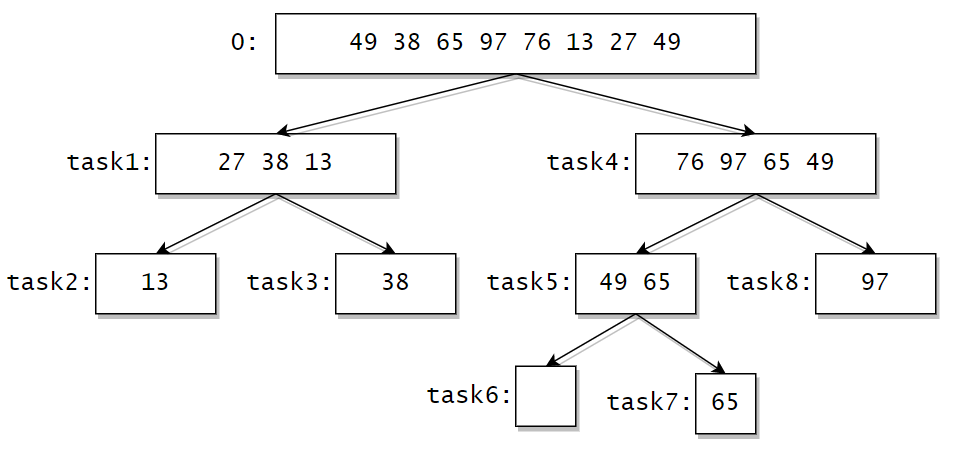
\includegraphics[scale=0.4]{openMP_quick_sort.png}
\caption{快速排序递归过程}
\label{fig:p1}
\end{figure}

我觉得递归树上的每一行的所有任务是可以并行执行的,如果线程调度比较合理,排序程序的时间复杂度最优可以达到$O(log_2n)$。task是“动态”定义任务的,在运行过程中,需要使用task就会定义一个任务,任务就会在一个线程上去执行,那么其它的任务就可以并行的执行。可能某一个任务执行了一半的时候,或者甚至要执行完的时候,程序可以去创建第二个任务,任务在一个线程上去执行,一个动态的过程。由于这些每个任务的执行时机不能确定,所以在并行化环境中时间复杂度可以达到$O(n)$,但是如果线程的数目不能满足递归树上的每一个结点,时间复杂度会增大但一定$\lesssim O(nlogn)$。

程序中仅开辟了一个一维数组对数据进行保存,空间复杂度为$O(n)$。

\subsubsection{实验结果和分析}
仍然使用之前的输入: 8 49 38 65 97 76 13 27 49

但由于任务执行或者说线程的调度的不确定性,其中间执行过程不一定每一次都是一样的,但是不论中间过程是怎样的,总体执行的流程还是与图\ref{fig:p1}所示的递归树一致。执行的结果是$\{13, 27, 38, 49, 49, 65, 76, 97\}$

\subsection{MPI环境下的并行排序算法设计}
\subsubsection{实验目的与要求}
编写使用MPI的C语言小程序,并按要求输出对应的排序后的结果。掌握MPI的基本知识以及使用方法。

\subsubsection{算法描述}
MPI是一个跨语言(编程语言如C, Fortran等)的通讯协议,用于编写并行计算机。支持点对点和广播。MPI是一个信息传递应用程序接口,包括协议和和语义说明,他们指明其如何在各种实现中发挥其特性。MPI的目标是高性能,大规模性,和可移植性。MPI在今天仍为高性能计算的主要模型。与OpenMP并行程序不同,MPI是一种基于信息传递的并行编程技术。消息传递接口是一种编程接口标准,而不是一种具体的编程语言。简而言之,MPI标准定义了一组具有可移植性的编程接口。

为了使用MPI的消息传递机制进行并行编程,我们在基本的快速排序程序上进行一层封装,在封装内部实现信息的通信以及对快速排序基本程序的调用。我们将这个函数命名为$quicksort\_recursive$,算法流程见算法\ref{alg:F4}。

\begin{algorithm}[htb]
\caption{quicksort\_recursive}
\label{alg:F4}
\hspace*{0.02in} {\bf Input:}
数组arr、数组大小 arrSize、当前进程号currProcRank、最大进程号maxRank、当前进程所在层号rankIndex\\
\hspace*{0.02in} {\bf Output:} 
无
  \begin{algorithmic}[1]
    \State
        计算与当前进程需要发送一半数据的进程号是多少;rankIndex加1表示移到下一层;如果计算出来的进程号大于最大进程号(目标进程不可用),则自己调用快速排序函数对arr数组进行排序
    \State
        如果计算出的目标进程号是可用的,则利用partition函数对arr进行划分,获取划分的基准值在arr中的索引pivotIndex。
    \State
        总是将两个划分中元素个数较少的子数组发送给目的进程;然后递归调用quicksort\_recursive,把剩下的子数组作为参数传入;最后接收被发出去的元素个数较少的子数组的数据(应当是已经排好序且通过某个进程发送过来的)。
  \end{algorithmic}
\end{algorithm}



下面对main函数的实现逻辑进行描述。总体的思路大致是通过0号进程进程数据的输入、数据最开始的分发以及数据最后的整合。

(1) \texttt{ 初始化MPI环境,获取当前进程号和进程数;}

(2) \texttt{ 判断当前进程的进程号是否为0,如是则读取用户输入数组的大小n以及数组元素(仅0号进程读取);}

(3) \texttt{ 对于所有的进程,计算进程号对应的递归树的层号,递归树的一个示例如图\ref{fig:p1}所示。然后通过调用MPI\_Barrier函数等待进程通信组中的所有进程到达这一点。}

(4) \texttt{ 判断当前进程的进程号是否为0,如是则调用快速排序子程序,将整个未排序的数组(unsorted\_arr)、其大小(n)、其进程号(rank)、最大进程号(size-1)、0号进程所在的层数(rankPow)作为参数;}

(5) \texttt{ 如果是其他进程,则使用MPI\_Probe函数先探测接收消息的内容,一旦检测到任何发送者发送给任何接收者的消息,使用结构体status接收有关消息的信息,包括其来源(source\_process)和大小(subarray\_size),其中大小使用MPI\_Get\_count函数通过传入status作为参数获得(实际上这里的消息就是子数组,大小就是子数组的元素个数)。利用获得的子数组的大小开辟一个缓冲区(subarray),然后使用MPI\_Recv函数接收子数组数据,放至定义好的缓冲区中,对缓冲区中的子数组调用快速排序子程序进行排序,参数为子数组(subarray)、子数组大小(subarray\_size)、当前进程号(rank)、最大进程号(size-1)、当前进程所在层数(rankPow),最后将排序后的子数组的数据发送给0号进程。}

(5) \texttt{ 数组排序完成,结束MPI通信进程。}



\subsubsection{复杂度分析}
使用MPI的消息通信机制的并行程序,其时间复杂度的大小与数组元素的个数和进程的数目有关,进程数目也不是越多越好,因为这样会加剧通信的开销以降低程序执行的效率。但不管怎样,该并行程序的时间复杂度一定$\lesssim O(nlogn)$。

程序中仅开辟了一个一维数组对数据进行保存,空间复杂度为$O(n)$。
\subsubsection{实验结果和分析}
假设指定的进程数目为4个(进程号为0-3),用户输入的数组数据仍然使用包含8个元素的49, 38, 65, 97, 76, 13, 27, 49。其执行过程如图\ref{fig:p2}所示

\begin{figure}[ht]
\centering
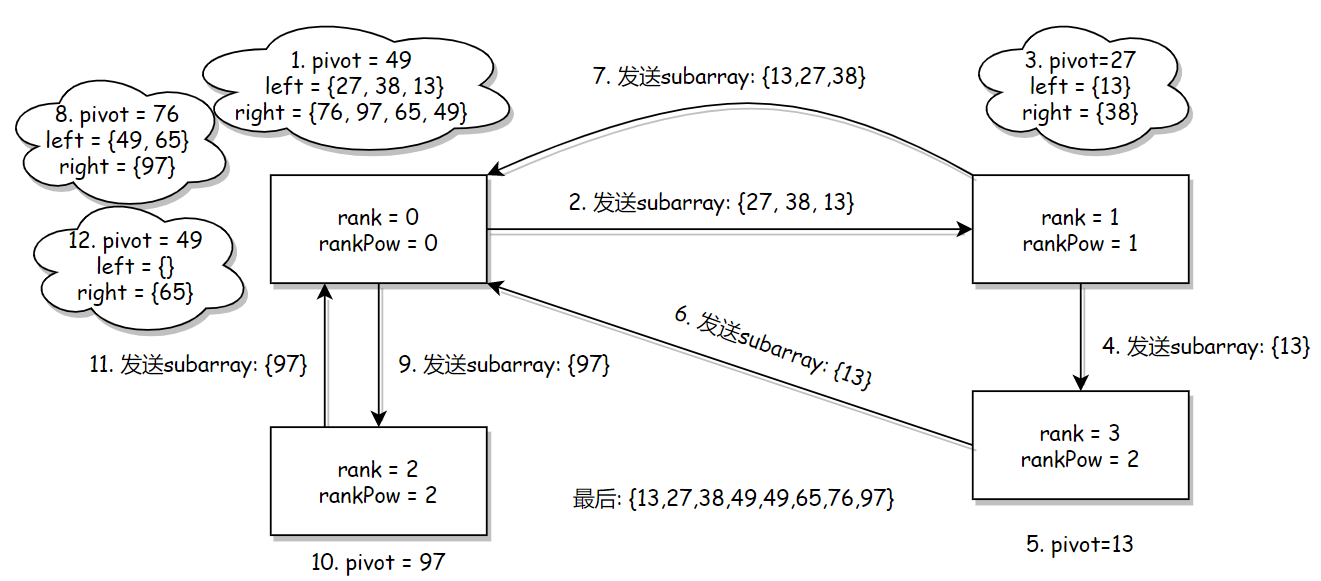
\includegraphics[scale=0.6]{MPI_quick_sort.png}
\caption{MPI快速排序并行执行过程}
\label{fig:p2}
\end{figure}

\newpage
\section{实验二}
\subsection{串行环境下的杨辉三角输出}
\subsubsection{实验目的与要求}
串行环境下编写打印杨辉三角形的C语言小程序,并按要求输出对应的杨辉三角形。本关需要掌握杨辉三角的基本格式。

\subsubsection{算法描述}
通过观察杨辉三角的数据排列方式,我们可以总结出以下规律:

(1) \texttt{杨辉三角的两个腰边上的数都是1;}

(2) \texttt{对于其他的位置:当前值 = 上一行前一列的值 + 上一行同一列的值。}

串行环境下的杨辉三角的计算的算法描述见算法\ref{alg:F5}。

\begin{algorithm}[htb]
\caption{串行环境下的杨辉三角输出}
\label{alg:F5}
\hspace*{0.02in} {\bf Input:}
需要输出的杨辉三角的层数n\\
\hspace*{0.02in} {\bf Output:} 
计算并打印层数为n的杨辉三角
  \begin{algorithmic}[1]
    \State
        初始化一个大小为$n\times n$的二维数组a,置a[i][0] = 1,a[i][i] = 1,其中$0\le i < n$,这个过程就是将杨辉三角的两个腰边上的数赋值为1。
    \State
        从左到右,从上到下对其他位置上的数进行计算,计算的公式为a[i][j] = a[i-1][j-1] + a[i-1][j],其中$2 \le i < n\ and\ 1 \le j < i$
    \State
        最后将杨辉三角按照格式进行输出即可。
  \end{algorithmic}
\end{algorithm}

\subsubsection{复杂度分析}
杨辉三角的空间复杂度等同于存储杨辉值的二维数组大小,所以空间复杂度为$O(n^2)$。
由于杨辉三角形中对于每个元素的计算都是常量时间,因此对于n层的杨辉三角形,其时间复杂度为$1+2+3+...+n=\sum_{i=1}^{n}i = \frac{n(n+1)}{2}$,即$O(n^2)$。

\subsubsection{实验结果和分析}
假设用户输入的层数n = 6,杨辉三角的计算过程和结果如图\ref{fig:p3}所示。

\begin{figure}[ht]
\centering
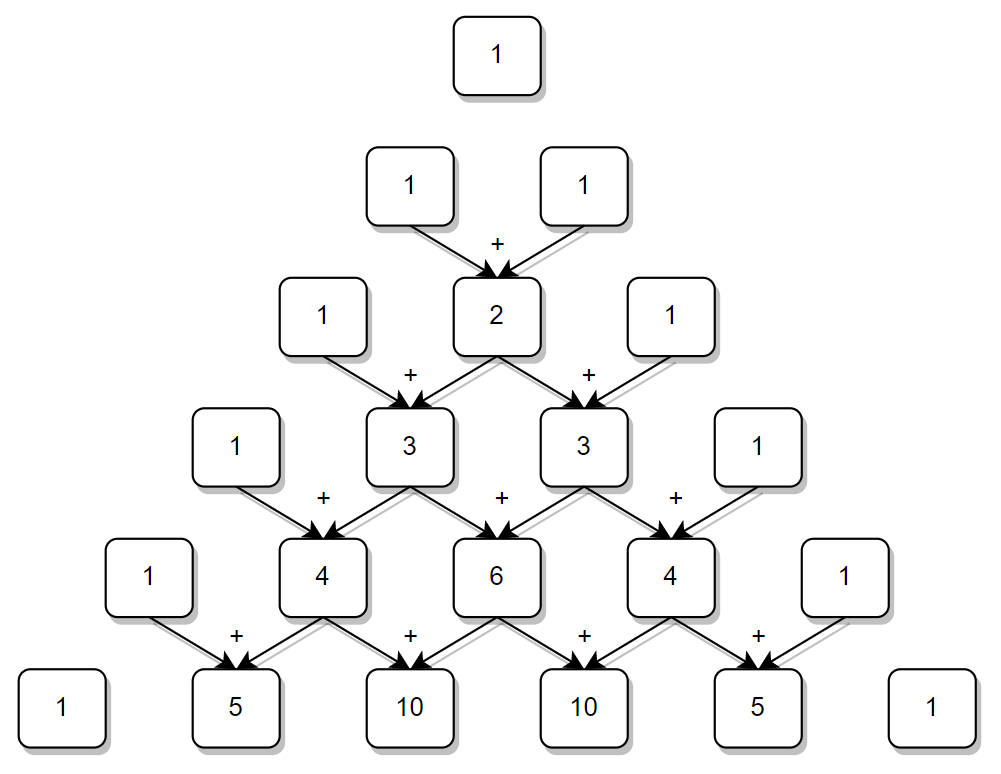
\includegraphics[scale=0.5]{杨辉三角.png}
\caption{杨辉三角计算过程}
\label{fig:p3}
\end{figure}


\subsection{OpenMP环境下的杨辉三角输出}
\subsubsection{实验目的和要求}
掌握OpenMP的基本知识和使用方法,编写使用OpenMP打印杨辉三角形的C语言小程序,并按要求输出对应的杨辉三角形。
\subsubsection{算法描述}
相比于实验一中的利用OpenMP实现并行快速排序,杨辉三角的计算过程可以并行的部分就在于两个for循环,因此我们需要使用能够对for循环有帮助的编译制导指令。对于指令\texttt{\#pragma omp parallel for},它表示接下来的for循环将被多线程执行。

但是OpenMP对于需要并行化的for循环有如下要求:

(1) \texttt{循环的变量变量(就是i)必须是有符号整形,其他的都不行;}

(2) \texttt{循环的比较条件必须是<、<=、>、>=中的一种;}

(3) \texttt{循环的增量部分必须是增减一个不变的值(即每次循环是不变的);}

(4) \texttt{如果比较符号是<、<=,那每次循环i应该增加,反之应该减小;}

(5) \texttt{循环不能从内部循环跳到外部循环,goto和break只能在循环内部跳转,异常必须在循环内部被捕获}

在串行环境下的杨辉三角形各个元素的计算方法已经在算法\ref{alg:F5}中给出,其中包含两个for循环,一个for循环对两个腰边直接赋值,另一个for循环计算杨辉三角内部的各个元素。由于这两个for循环都符合OpenMP并行化的for循环条件,因此我们只需要在两个for循环语句的上面添加编译制导指令\texttt{\#pragma omp parallel for}即可。不过在并行程序执行之前,首先需要设置执行并行代码的线程数目,我在实验的过程中设置的是4个线程。

\subsubsection{复杂度分析}
使用for制导语句会将for循环拆开来尽可能平均的分配到各个线程进行执行,因此假设线程的个数为K,串行计算杨辉三角形的时间复杂度为$O(n^2)$,则多个线程并行执行for循环的时间复杂度为$O(\frac{n^2}{K})\lesssim O(n^2)$

杨辉三角的空间复杂度等同于存储杨辉值的二维数组大小,所以空间复杂度为$O(n^2)$。
\subsubsection{实验结果和分析}
假如用户希望输出的杨辉三角的层数为6,无论线程如何分配执行,总体的执行流程仍然与图\ref{fig:p3}一致。最后结果都会是[[1], [1, 1], [1, 2, 1], [1, 3, 3, 1], [1, 4, 6, 4, 1], [1, 5, 10, 10, 5, 1]]。

\subsection{MPI环境下的杨辉三角输出}
\subsubsection{实验目的与要求}
掌握MPI的基本知识和使用方法,编写使用MPI打印杨辉三角形的C小程序,并按要求输出对应杨辉三角形。
\subsubsection{算法描述}
对于如何使用MPI对杨辉三角进行并行计算,我参考了一个网站上面的例子,网址为\href{}{https://daugerresearch.com/vault}。由于之前的串行计算杨辉三角的程序不好拆解,我首先对串行程序进行了改写,为后续的并行编程做准备。改写后的串行程序为了节省空间,仅使用了一个一维数组对结果进行保存。下面介绍改写后串行程序的基本函数:

(1) \texttt{addright \& addleft: 这两个函数都可以执行一维数组中相邻元素相加的操作,其结果仍然放至该一维数组中,以节省内存分配和内存访问。通过交替调用addleft和addright函数可以避免潜在的内存移动和复制操作。}

(2) \texttt{iterationloop: 该函数在指定次数的迭代中执行循环,交替调用addleft和addright函数,如果循环次数为奇数则调用addleft,如果循环次数为偶数则调用addright。}

(3) \texttt{computeloop: 分配内存,对一维数组进行初始化,调用iterationloop函数,并将最后一维数组的结果进行返回。}

(4) \texttt{main: 调用computeloop函数,获得最终结果,最后释放内存。}

上述串行计算杨辉三角的程序的执行步骤,其实就是把二维数组压缩成一维数组,然后直接利用上一行的计算结果计算这一行的数据,结果保存在同一个一维数组中,利用的是杨辉三角内部元素当前值 = 上一行前一列的值 + 上一行同一列的值这个特性。假设打印杨辉三角的层数为6,则程序一维数组的大小将会为7,该串行程序的计算杨辉三角的过程如图\ref{fig:p4}所示。

\begin{figure}[ht]
\centering
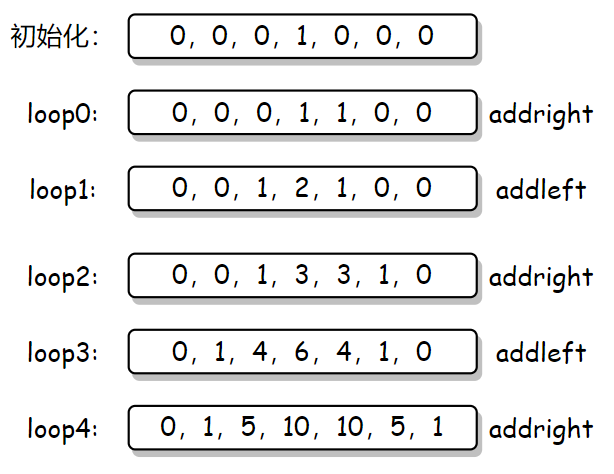
\includegraphics[scale=0.8]{杨辉三角01.png}
\caption{一维数组的杨辉三角计算过程}
\label{fig:p4}
\end{figure}

接下来在上述串行程序的基础上使用MPI进行并行编程。大致的思路就是将整行一维数组平均分配给每个处理器,不同的处理器处理不同的分区,处理器之间相互传递消息,以保证数据计算的正确性。如算法\ref{alg:F6}所示。

\begin{algorithm}[htb]
\caption{MPI环境下的杨辉三角输出}
\label{alg:F6}
\hspace*{0.02in} {\bf Input:}
需要输出的杨辉三角的层数n\\
\hspace*{0.02in} {\bf Output:} 
计算并打印层数为n的杨辉三角
  \begin{algorithmic}[1]
    \State
        main:MPI初始化将当前处理器id以及处理器个数保存至idproc和nproc变量中。仅0号处理器读取用户的输入n,并利用MPI\_Bcast函数将该变量的值广播给所有处理器。调用computeloop函数,n,nproc以及idproc作为参数。
    \State
        computeloop:根据n和nproc的大小对每个处理器需要处理的任务(数据量)进行划分。如果是0号处理器,则开辟一个大数组的空间用于整合所有分任务的计算结果;对于其他的处理器,根据划分的任务数据量大小开辟空间。对数组进行初始化操作,即将数组中间某个元素赋值为1,其余全部赋值为0。调用iterationloop函数,将任务数组、数组的大小、输出层数n、idproc以及nproc作为参数。
    \State
        iterationloop:首先指定leftIDProc和RightIDProc表示用于通信的处理器ID编号。然后对任务数组进行迭代循环,循环的次数即为输出的层数。
    \State
        如果循环次数为奇数则调用addleft函数,然后从rightIDProc接收任务数组最右边的元素,将本任务数组左边的元素发送给leftIDProc,使用MPI\_Wait函数确保数据进行了传输。
    \State
        对于循环次数为偶数的情况则调用addright,然后从leftIDProc接收任务数组最左边的元素,发送任务数组最右边的元素给rightIDProc,使用MPI\_Wait函数确保数据进行了传输。
    \State
        由于需要打印每一次迭代的结果数据,需要在iterationloop中利用MPI\_Gather函数,将所有处理器的任务数组数据整合到0号处理器的大数组中。
  \end{algorithmic}
\end{algorithm}

下面对算法\ref{alg:F6}中提及的一些变量和函数及其作用进行说明:

(1) \texttt{idproc, nproc: nproc描述当前有多少处理器正在运行此作业,idproc标识处理器的名称(0~nproc-1)。这两个变量由main提供给computeloop函数,由computeloop函数提供给iterationloop函数。}

(2) \texttt{leftIDProc \& rightIDProc: 该变量描述了所指定的左右相邻的处理器ID,用于迭代循环内的通信,在迭代循环进行之前进行计算。}

(3) \texttt{MPI\_Irecv, MPI\_Send, and MPI\_Wait: 这些是基本的MPI接口,将一个处理器的结果数据与另一个处理器的初始数据连接起来。leftIDProc和RightIDProc标识消息发送和接收的处理器ID。}

(4) \texttt{iterationloop函数被赋予一个数组,该数组比该处理器实际负责的空间要大一个元素,额外的元素用作“保护”元素。保护元素位于分区的右边缘。addleft之后,将该处理器最左边的元素通过MPI\_Send提供给左边的处理器,该处理器最右边的元素通过MPI\_Recv从右边的处理器获得。addright之后,使用MPI\_Send将此处理器最右侧的元素发送给右侧相邻的处理器,此处理器最左侧的元素通过使用MPI\_Recv接收来自左侧相邻处理器的消息获得。}

\subsubsection{复杂度分析}
本实验将杨辉三角的计算从二维数据压缩到了一维数组,因此空间复杂度为$O(n)$。

尽管并行程序的执行使用多处理器,但由于MPI的处理器通信机制也会带来一定的开销,处理器的数目以及数组大小的相对性也会对程序的执行时间有影响。在这里只能带有前提假设的给出MPI并行环境下时间复杂度的估计值,假设处理器的个数为K,且任务分配均匀,则时间复杂度为$O(\frac{n^2}{K})\lesssim O(n^2)$。

\subsubsection{实验结果和分析}
MPI环境下的杨辉三角的计算过程如图\ref{fig:p5}所示。图中每一行代表一次迭代过程,红色的箭头表示消息传递方向,这张图也表明了addright和addleft的交替执行过程。
\begin{figure}[ht]
\centering
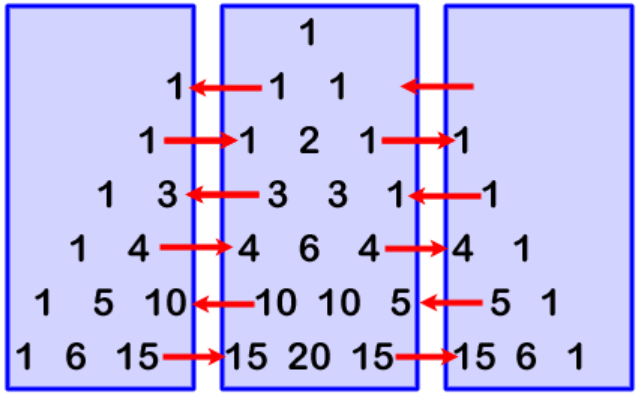
\includegraphics[scale=0.7]{杨辉三角02.png}
\caption{MPI环境下杨辉三角计算过程}
\label{fig:p5}
\end{figure}

\newpage
\section{总结}
通过并行编程原理与实践课程,我学习到了许多之前完全没有接触到的新鲜事物,对于并行处理的底层实现机制也有了自己的理解,通过实践课程我也掌握了pthread、OpenMP以及MPI环境下并行编程的具体实现方法。

MPI实质上是多进程,并且不支持多线程;初始化时在每个处理机上创建一个进程,执行期间进程数目不能动态改变;MPI其实就是一种在各个进程之间进行通讯的标准。

多核下的多线程程序设计需要将应用程序看做是众多相互依赖的任务集合,将应用程序划分为多个独立的任务,并确定这些任务之间的相互依赖关系,这就称为分解。包括任务的分解、数据的分解、数据流的分解:

(1) \texttt{任务分解:对应用程序根据其执行的功能进行分解的过程;}

(2) \texttt{数据分解:数据级并行,将应用程序根据各任务所处理的数据而非按任务来进行分解;}

(3) \texttt{数据流分解:基于数据在这些任务之间是如何流动的进行分解。}

多线程程序设计中,线程的数目不是越多越好,对于某个程序,如果线程过多反而会严重地降低程序的性能。这种影响主要在于:将给定的工作量划分给过多的线程会造成每个线程的工作量过少,导致线程启动和终止的开销比程序实际工作的时间还要多。同时太多并发线程的存在将导致共享有限硬件资源的开销增大。如保存和恢复寄存器状态的开销、保存和恢复线程cache状态的开销、废除虚存的开销。

因此在进程并行程序的设计时,我们需要考虑很多问题,以便获得更好的程序执行效果。想要熟练的掌握并行编程的方法,还需要更多的学习和实践。

最后我想给本课程提一个小建议:我认为实验课程可能与理论课程可以同步进行,这样大家的学习效果和实践效果会更好。

在这里教你怎么引用:\cite{ref1}

\begin{thebibliography}{99}  

\bibitem{ref1}Durgam S, Earley W, Lipschitz A, et al. An 8-week randomized, double-blind, placebo-controlled evaluation of the safety and efficacy of cariprazine in patients with bipolar I depression[J]. American Journal of Psychiatry, 2016, 173(3): 271-281.

\end{thebibliography}


\section*{\zihao{4} 华中科技大学本科生毕业设计(论文)开题报告评审表}
\thispagestyle{empty}
% Please add the following required packages to your document preamble:
% \usepackage{multirow}
% \usepackage[table,xcdraw]{xcolor}
% If you use beamer only pass "xcolor=table" option, i.e. \documentclass[xcolor=table]{beamer}

\begin{table}[htbp]

\resizebox{150mm}{93mm}{
\setlength{\tabcolsep}{10mm}{

\begin{tabular}{|cccccc|}
\hline
\multicolumn{1}{|c|}{\textbf{姓名}} & \multicolumn{1}{c|}{\textbf{}} & \multicolumn{1}{c|}{\textbf{学号}} & \multicolumn{1}{c|}{\textbf{}} & \multicolumn{1}{c|}{\textbf{指导教师}} & \textbf{} \\ \hline
\multicolumn{2}{|c|}{\textbf{院(系)专业}}                              & \multicolumn{4}{c|}{\textbf{}}                                                                                     \\ \hline
\multicolumn{6}{|c|}{\textbf{指导教师评语}}       \\                                                                            \multicolumn{6}{|l|}{{1.学生前期表现情况。}}    \\

\multicolumn{6}{|l|}{{2.是否具备开始设计(论文)条件?是否同意开始设计(论文)? }}   \\
\multicolumn{6}{|l|}{{3.不足与建议。}}  \\
\hline
\multicolumn{6}{|c|}{{\color[HTML]{FF0000} }}                                                                                                                                           \\
\multicolumn{6}{|c|}{{\color[HTML]{FF0000} }}                                                                                                                                           \\
\multicolumn{6}{|c|}{{\color[HTML]{FF0000} }}                                                                                                                                           \\
\multicolumn{6}{|c|}{{\color[HTML]{FF0000} }}                                                                                                                                           \\
\multicolumn{6}{|c|}{{\color[HTML]{FF0000} }}                                                                                                                                           \\
\multicolumn{6}{|c|}{{\color[HTML]{FF0000} }}                                                                                                                                                                                                                    \\
\multicolumn{6}{|c|}{{\color[HTML]{FF0000} }}                                                                                                                                           \\
\multicolumn{6}{|c|}{{\color[HTML]{FF0000} }}                                                                                                                                           \\
\multicolumn{6}{|c|}{\multirow{-15}{*}{{\color[HTML]{FF0000} }}}                                                                                                                        \\ \hline
\multicolumn{6}{|l|}{}                                                                                                                                                                  \\
\multicolumn{6}{|l|}{\multirow{-2}{*}{指导教师(签名):}}                                                                                                                                       \\ 
\multicolumn{6}{|r|}{年\qquad 月\qquad 日}                                                                                                                                                       \\ \hline
\multicolumn{6}{|c|}{\textbf{教研室(系、所)或开题报告答辩小组审核意见}}                                                                                                                                    \\ \hline
\multicolumn{6}{|c|}{{\color[HTML]{FF0000} }}                                                                                                                                           \\
\multicolumn{6}{|c|}{{\color[HTML]{FF0000} }}                                                                                                                                           \\
\multicolumn{6}{|c|}{{\color[HTML]{FF0000} }}                                                                                                                                           \\
\multicolumn{6}{|c|}{{\color[HTML]{FF0000} }}                                                                                                                                           \\
\multicolumn{6}{|c|}{\multirow{-5}{*}{{\color[HTML]{FF0000} }}}                                                                                                                         \\ \hline
\multicolumn{6}{|l|}{}                                                                                                                                                                  \\
\multicolumn{6}{|l|}{\multirow{-2}{*}{教研室(系、所)或开题报告答辩小组负责人(签名):}}                                                                                                                       \\ 
\multicolumn{6}{|r|}{年\qquad 月\qquad 日}                                                                                                                                                       \\ \hline
\end{tabular}
}
}

\end{table}
\end{document}
